\chapter{Air Shower Physics}


Above energies of 100 TeV (10$^{14}$ eV) direct detection becomes increasingly difficult \cite{RevModPhys.71.S165}. Ground based observations are made by exploiting extensive air showers (EAS). EAS were first discovered by Pierre Auger in 1932 when noticed that cosmic-rays were arriving at different detectors at the same time. He formed the conclusion that they were secondary particles emitted from the same source \cite{RevModPhys.11.288}.

An extensive air shower is a cascade of secondary particles that begins when the cosmic ray
first interacts with the earth’s atmosphere. Three main components of an extensive air shower are:

\begin{itemize}
\item Electromagnetic - consisting of electrons, positrons and $\gamma$-rays resulting from the decay of charged and neutral pions and kaons.
\item Hadronic component - consisting of heavy nuclei, charged pions and kaons.
\item Muonic - consisting of muons and neutrinos resulting from the decay of charged pions and kaons.
\end{itemize}

The height at which cosmic rays interact within the atmosphere is dependent on their energy and composition. A measure of the amount of atmospheric matter above ground level is called the atmospheric or slant depth $X$. The unit of slant depth is usually g/cm$^2$. To calculate the slant depth, firstly need to define a vertical atmospheric depth.
\begin{equation}
X_v = \int^{\infty}_{h} \rho(h')\diff h'
\end{equation}
where $X_v$ is the vertical atmospheric depth and $\rho$ is the atmospheric density. Now a slant depth can be defined.  
\begin{equation}
X = \frac{X_v}{\mathrm{cos}(\theta)}
\end{equation}
where $\theta$ is the angle from the zenith. Shower age $s$ is a parameter often used to describe the development of an extensive air shower relative to shower maximum. The slant depth at which shower maximum occurs is defined as depth of maximum development ($X_{max}$). Shower age is defined as
\begin{equation}
s(X) = \frac{3}{(1 + 2 X_{max} / X)}
\end{equation}

\section{Electromagnetic Component}

\begin{figure}[htp]
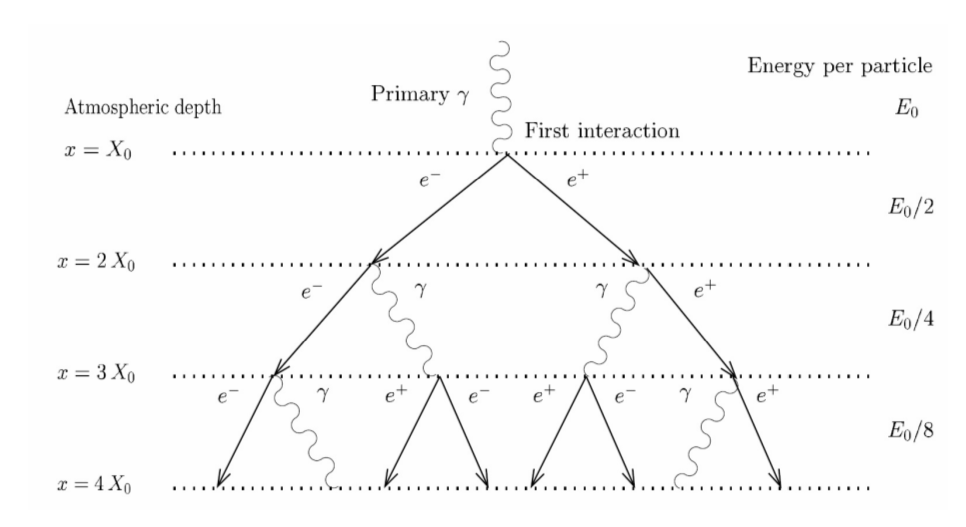
\includegraphics[width=\textwidth]{../pictures/heilter_model_EM.png}
\caption{A graphical representation of the Heitler model.}\label{fig:heitler_model}
\end{figure}

To describe the electromagnetic shower, a simple model was proposed by Heitler \cite{Heitler}. In this model a $\gamma$-ray of $E_0$ interacts with an atmospheric nucleus (N), creating an electron-positron pair via pair-production
\begin{equation}
\gamma + N \rightarrow e^+ + e^- 
\end{equation}
Each of the electron and positron then give half of their energy to $\gamma$-ray via bremsstrahlung
\begin{equation}
e^{\pm} + N \rightarrow N + e^{\pm} + \gamma
\end{equation}
This process continues as shown in Figure \ref{fig:heitler_model} until the energy of the particles falls below the critical energy $E_C$ required for further particle production, and ionisation begins to dominate.

The energy of each shower particle after $n$ radiation lengths will be
\begin{equation}
E(n) = \frac{E_0}{2^n}
\end{equation}

Once the individual particles energy drops below the energy where ionisation dominates no more particles are produced. Therefore the maximum particle number is
\begin{equation}
N_{max} = \frac{E_0}{E_C}
\end{equation}

\section{Hadronic Component}

\begin{figure}[htbp]
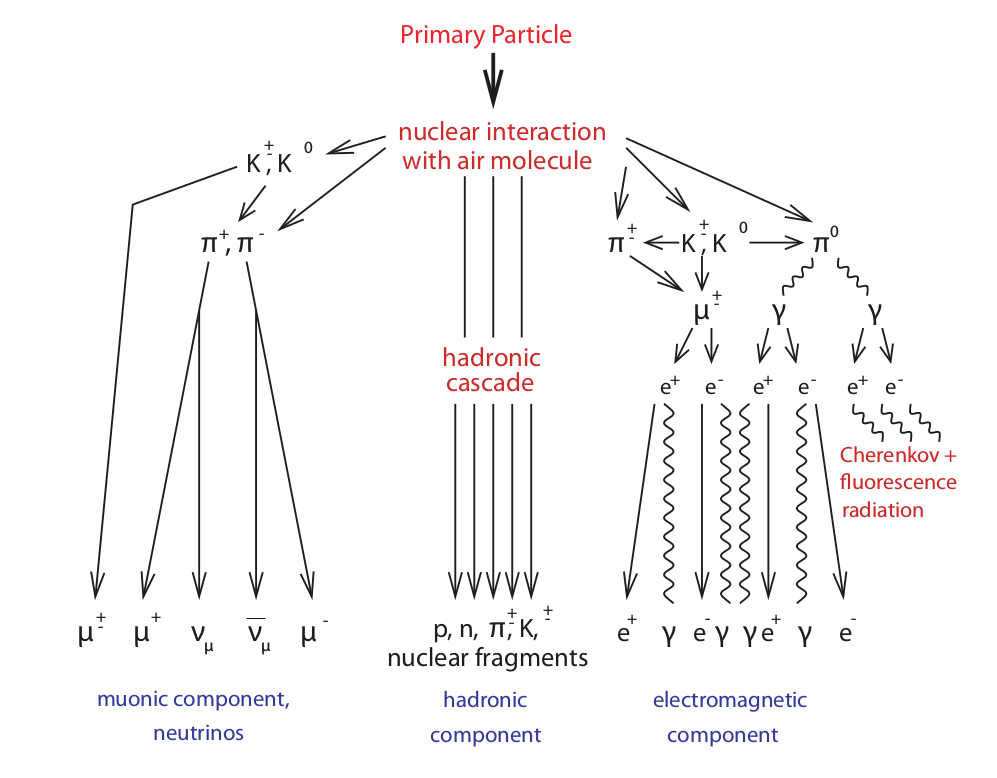
\includegraphics[width=\textwidth]{../pictures/hielter_model_hadronic.png}
\caption{A graphical representation of the Heitler model for an extensive air shower initiated by a hadronic primary. Image taken from \cite{0034-4885-66-7-202}.}
\end{figure}

A hadronic EAS is initiated the same way in the atmosphere as a electromagnetic shower but the interaction produces kaons and charged and neutral pions \cite{kumpel}. An approach similar to Heitler's treatment of electromagnetic cascades can be used to explain the basic properties of hadronic cascades. The atmospheric is divided into layers, with the thickness of each layer characterised by an interaction length $\lambda_I$. After travelling one interaction length, the primary hadron interacts with the atmosphere and produces $2N$ charged pions and $N$ neutral pions. The neutral pions decay into two photons
\begin{equation}
\pi^0 \rightarrow \gamma + \gamma
\end{equation}
These photons can initiate electromagnetic cascades, and the charged pions becoming the next generation of the hadronic shower. The process continues until the energy of the pions drops below a critical energy $E^I_{crit} \approx$ 20 GeV. The critical energy is the point where the decay length becomes shorter than the interaction length. At this threshold, the charged pions decay
\begin{eqnarray}
\pi^+ & \rightarrow & \mu^+ + \nu_{\mu} \\
\pi^- & \rightarrow & \mu^- + \bar{\nu}_{\mu}
\end{eqnarray}
